\documentclass[10pt,
               a4paper,
               journal,
               ]{IEEEtran}
\makeatletter

\def\markboth#1#2{\def\leftmark{\@IEEEcompsoconly{\sffamily}\MakeUppercase{\protect#1}}%
\def\rightmark{\@IEEEcompsoconly{\sffamily}\MakeUppercase{\protect#2}}}
\makeatother

\usepackage[utf8]{inputenc}
\usepackage[T1]{fontenc}
\usepackage{cite}
\usepackage{amsfonts}
\usepackage[pdftex]{graphicx}
\graphicspath{{../png/}}
\DeclareGraphicsExtensions{.png}
\usepackage[cmex10]{amsmath}
\interdisplaylinepenalty=2500
\usepackage{array}
\usepackage{mdwmath}
\usepackage{mdwtab}
\usepackage{eqparbox}
\usepackage[caption=false,font=footnotesize]{subfig}
\usepackage{fixltx2e}
\usepackage{stfloats}
\usepackage{url}
\hyphenation{op-tical net-works semi-conduc-tor}
\usepackage{stmaryrd}
\usepackage{bbding}
\usepackage{algpseudocode}
\usepackage{algorithm}
\usepackage{tikz}
\usetikzlibrary{shapes}
\usetikzlibrary{calc}
\usetikzlibrary{positioning}
\usetikzlibrary{patterns}
\usepackage{listings}
\usepackage{color}

\definecolor{dkgreen}{rgb}{0,0.6,0}
\definecolor{gray}{rgb}{0.5,0.5,0.5}
\definecolor{mauve}{rgb}{0.58,0,0.82}

\lstset{frame=tb,
  language=C++,
  aboveskip=3mm,
  belowskip=3mm,
  showstringspaces=false,
  columns=flexible,
  basicstyle={\small\ttfamily},
  numbers=none,
  numberstyle=\tiny\color{gray},
  keywordstyle=\color{blue},
  commentstyle=\color{dkgreen},
  stringstyle=\color{mauve},
  breaklines=true,
  breakatwhitespace=true
  tabsize=3
}

\newcommand{\reffig}[1]{{figure \ref{#1}}}
\newcommand{\refeq}[1]{{(\ref{#1})}}

\begin{document}
	\title{Constraint Programming - Inside Gecode}
	\author{Benedikt~Schmidt}
	\markboth{Advanced Seminar for Security in Information Technology, Summer Term 2014}%
	{Benedikt Schmidt: Constraint Programming - Inside Gecode}	
	\maketitle	
	
	\begin{abstract}	
		Constraint programming is a way to describe and solve mathematical problems with arbitrary constraints. In the following paper I will explain the implemented algorithms in Gecode, a tool which can be used to solve problems through constraint programming.
	\end{abstract}
	
	\section{Introduction}
	Constraint programming is a method to solve mathematical problems through the formulation of constraints, which describe the desired solution. As a formal and exact definition, like it can be found in \cite[p.~16]{handbookCP} for constraint programming, is not as helpful as an example, I would like to give you a short overview on the topic through the problem of the placement of two squares such that they do not overlap.	
	
	\begin{figure}
		\center
		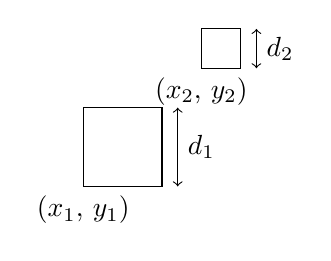
\begin{tikzpicture}
			\draw (0, 0) rectangle (1, 1);
			\node at (0, -0.3) {($x_1$, $y_1$)};
			\draw[arrows=<->] (1.2, 0) -- (1.2, 1);
			\node at (1.5, 0.5) {$d_1$};
			\draw (1.5, 1.5) rectangle(2, 2);
			\node at (1.5, 1.2) {($x_2$, $y_2$)};
			\draw[arrows=<->] (2.2, 1.5) -- (2.2, 2);
			\node at (2.5, 1.75) {$d_2$};
		\end{tikzpicture}
		\caption{two squares which should not overlap}
		\label{fig:squares}
	\end{figure}
	
	The related variables for this example are defined in \reffig{fig:squares}. The problem can be expressed by \cite[p. 101]{programmingGecode}
	\begin{equation}
	\begin{split}
		x_1 + d_1 \le x_2 & \lor x_2 + d_2 \le x_1 \lor \\
		y_1 + d_1 \le y_2 & \lor y_2 + d_2 \le y_1
	\end{split}
	\label{eq:squares}
	\end{equation}
	The task for the constraint programming tool at this point is then to find feasible solutions which fulfill the constraints.
	
	A solver for constraint programming like \emph{Gecode} provides the necessary tools to define constraints like \refeq{eq:squares} in their most natural form as equations and inequations and will find all possible solutions or just one of them, depending on the selected algorithm. If there would be only linear constraints like it would be possible to solve this problem through linear programming \cite[1]{linearProgramming}. As linear programming is only a subset of constraint programming the latter one is the more general one with more practical applications; not every problem in the real world is linear or can be linearized in a useful way. Consequently, constraint programming with its ability to consider constraints in their most general form can be used in various fields like scheduling of resources, computer-aided design and robotics \cite[p.~221]{trendsInCP}.
	
	In the following I will describe the necessary steps to solve a problem with constraint programming and as example of an implementation I will always refer to \emph{Gecode} \cite{gecode}.
	
	\section{State of the Art}
	\subsection{Variable Domains}
	In constraint programming a variable is connected to a set of possible values, the so called domain. Depending on the domain a variable is called an integer, boolean or floating variable. Possible ranges for a variable $x$ of each domain are:
	\begin{itemize}
		\item Integer: finite or inifnite sets like $x \in \mathbb{N}$, $x \in \{-5, 4, 10\}$, \dots
		\item Bool: $x \in \{\text{true}, \text{false}\}$
		\item Float: intervals or unions of intervals like $x \in [-4, 3]$, $x \in [-10, 8] \cup [10, 12]$, \dots
	\end{itemize}
	This distinction is fundamental as especially for floating variables the classical combinatorial approach to constraint programming is impossible.
	
	\subsection{Constraint Types}
	
	As constraint programming is the generalization of linear programming it is at least possible to define linear constraints. Which statements are possible to make and how handy it is to do so varies from the programming language in which the problem is implemented and the used toolset. Typical constraints are
	\begin{itemize}
		\item Equalities: $x = y + 2$, $x^2 + y^2 = 1$, \dots
		\item Inequalities: $x \ne y$, \dots
		\item Relations: $x < 2 y$, $e^x < 4$, \dots
	\end{itemize}
	
	Different constraint types can also be combined, for example inequalities or equalities through logic operators to boolean expressions. Some of these constraints may acquire special attention during the search for solutions to improve the execution reason. For this reason a lot of work has been done for example on the alldifferent constraint \cite{allDifferent}, which would be such a combined constraint.
	\begin{equation}
		\forall x_i, x_j \in D, i \ne j: x_i \ne x_j, 
		\label{eq:alldifferent}
	\end{equation}
	
	\subsection{Search Trees}
	
	\begin{figure}
		\center
		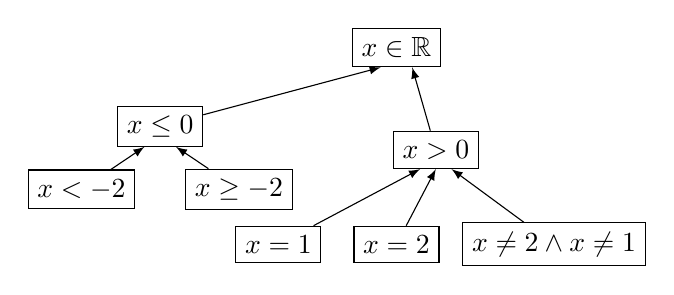
\begin{tikzpicture}
			\tikzstyle{arrow}=[draw, -latex]
			\node[rectangle,draw] at (0, 2) (levelOne) {$x \in \mathbb{R}$};
			
			\node[rectangle,draw] at (-3, 1) (levelTwoElementOne) {$x \le 0$};
			\coordinate[left=0.2cm of levelOne.south] (levelOnePointOne);
	  		\path[arrow] (levelTwoElementOne) -- (levelOnePointOne);
	  		
			\node[rectangle,draw] at (0.5, 0.7) (levelTwoElementTwo) {$x > 0$};
			\coordinate[right=0.2cm of levelOne.south] (levelOnePointTwo);
	  		\path[arrow] (levelTwoElementTwo) -- (levelOnePointTwo);
	  		
			\node[rectangle,draw] at (-4, 0.2) (levelThreeElementOne) {$x < -2$};
			\coordinate[left=0.2cm of levelTwoElementOne.south] (levelTwoElementOnePointOne);
	  		\path[arrow] (levelThreeElementOne) -- (levelTwoElementOnePointOne);
	  		
			\node[rectangle,draw] at (-2, 0.2) (levelThreeElementTwo) {$x \ge -2$};
			\coordinate[right=0.2cm of levelTwoElementOne.south] (levelTwoElementOnePointTwo);
	  		\path[arrow] (levelThreeElementTwo) -- (levelTwoElementOnePointTwo);
	  		
			\node[rectangle,draw] at (-1.5, -0.5) (levelThreeElementThree) {$x = 1$};
			\coordinate[left=0.2cm of levelTwoElementTwo.south] (levelTwoElementTwoPointOne);
	  		\path[arrow] (levelThreeElementThree) -- (levelTwoElementTwoPointOne);
	  		
			\node[rectangle,draw] at (0, -0.5) (levelThreeElementFour) {$x = 2$};
			\coordinate[right=0cm of levelTwoElementTwo.south] (levelTwoElementTwoPointTwo);
	  		\path[arrow] (levelThreeElementFour) -- (levelTwoElementTwoPointTwo);
	  		
			\node[rectangle,draw] at (2, -0.5) (levelThreeElementFive) {$x \ne 2 \land x \ne 1$};
			\coordinate[right=0.2cm of levelTwoElementTwo.south] (levelTwoElementTwoPointThree);
	  		\path[arrow] (levelThreeElementFive) -- (levelTwoElementTwoPointThree);
		\end{tikzpicture}
		\caption{search tree on one variable $x$}
		\label{fig:searchTree}
	\end{figure}
	
	In constraint programming search trees, like the one in \reffig{fig:searchTree}, describe the partition of the search space and their nodes have names, depending on position in the tree. The root node is the one from where the search is started and all variable domains are still complete. This one is also the first one with a branch, where for the first time the search space is split up into disjoint sets. This approach is similiar to the divide-and-conquer technique as it reduces a complex problem into two or more parts with less complexity. The splitting, which adds additional constraints on the variables, is then recursively done with different heuristics to partition the search space into smaller parts. If one of the parts is small enough to decide if it is feasible the node can be called a either a deadend or a solution. To end up as the dead end there must be no feasible solutions left in the search space at this node. To turn the node into a solution it is necessary that all members of the reduced search space are valid considering the constraints.
	
	\subsection{Constraint Propagation}
	Constraint propagation is a key concept in constraint programming as it reduces the size of the search space significantly. The term propagation refers in this area to the reduction of domains of variables which are infeasible, considering other constraints and affected variable domains. As the size of the variable domain is related to possibilities which have to be checked by a search, the constraint propagation is able to prune complete infeasible subtrees. Therefore the whole search process can be accelerated through constraint propagation.
	
	\begin{figure}
		\center
		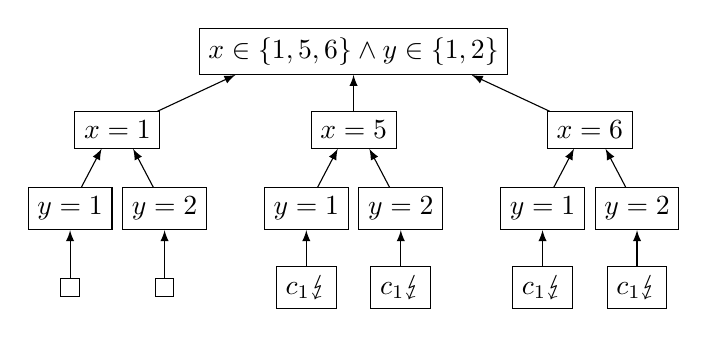
\begin{tikzpicture}
			\tikzstyle{arrow}=[draw, -latex]
			\node[rectangle,draw] at (0, 3) (levelOne) {$x \in \{1, 5, 6\} \land y \in \{1, 2\}$};
			
			\node[rectangle,draw] at (-3, 2) (levelTwoElementOne) {$x = 1$};
			\coordinate[left=1.5cm of levelOne.south] (levelOnePointOne);
	  		\path[arrow] (levelTwoElementOne) -- (levelOnePointOne);
	  		
			\node[rectangle,draw] at (0, 2) (levelTwoElementTwo) {$x = 5$};
			\coordinate[left=0cm of levelOne.south] (levelOnePointTwo);
	  		\path[arrow] (levelTwoElementTwo) -- (levelOnePointTwo);
	  		
			\node[rectangle,draw] at (3, 2) (levelTwoElementThree) {$x = 6$};
			\coordinate[right=1.5cm of levelOne.south] (levelOnePointThree);
	  		\path[arrow] (levelTwoElementThree) -- (levelOnePointThree);
	  		
			\node[rectangle,draw] at (-3.6, 1) (levelThreeElementOne) {$y = 1$};
			\coordinate[left=0.2cm of levelTwoElementOne.south] (levelTwoElementOnePointOne);
	  		\path[arrow] (levelThreeElementOne) -- (levelTwoElementOnePointOne);
			\node[rectangle,draw] at (-3.6, 0) (levelFourElementOne) {\Checkmark};
	  		\path[arrow] (levelFourElementOne) -- (levelThreeElementOne);
			\node[rectangle,draw] at (-2.4, 1) (levelThreeElementTwo) {$y = 2$};
			\coordinate[right=0.2cm of levelTwoElementOne.south] (levelTwoElementOnePointTwo);
	  		\path[arrow] (levelThreeElementTwo) -- (levelTwoElementOnePointTwo);
			\node[rectangle,draw] at (-2.4, 0) (levelFourElementTwo) {\Checkmark};
	  		\path[arrow] (levelFourElementTwo) -- (levelThreeElementTwo);
	  		
			\node[rectangle,draw] at (-0.6, 1) (levelThreeElementThree) {$y = 1$};
			\coordinate[left=0.2cm of levelTwoElementTwo.south] (levelTwoElementTwoPointOne);
	  		\path[arrow] (levelThreeElementThree) -- (levelTwoElementTwoPointOne);
			\node[rectangle,draw] at (-0.6, 0) (levelFourElementThree) {$c_1 \lightning$};
	  		\path[arrow] (levelFourElementThree) -- (levelThreeElementThree);
			\node[rectangle,draw] at (0.6, 1) (levelThreeElementFour) {$y = 2$};
			\coordinate[right=0.2cm of levelTwoElementTwo.south] (levelTwoElementTwoPointTwo);
	  		\path[arrow] (levelThreeElementFour) -- (levelTwoElementTwoPointTwo);
			\node[rectangle,draw] at (0.6, 0) (levelFourElementFour) {$c_1 \lightning$};
	  		\path[arrow] (levelFourElementFour) -- (levelThreeElementFour);
	  		
			\node[rectangle,draw] at (2.4, 1) (levelThreeElementFive) {$y = 1$};
			\coordinate[left=0.2cm of levelTwoElementThree.south] (levelTwoElementThreePointOne);
	  		\path[arrow] (levelThreeElementFive) -- (levelTwoElementThreePointOne);
			\node[rectangle,draw] at (2.4, 0) (levelFourElementFive) {$c_1 \lightning$};
	  		\path[arrow] (levelFourElementFive) -- (levelThreeElementFive);
			\node[rectangle,draw] at (3.6, 1) (levelThreeElementSix) {$y = 2$};
			\coordinate[right=0.2cm of levelTwoElementThree.south] (levelTwoElementThreePointTwo);
	  		\path[arrow] (levelThreeElementSix) -- (levelTwoElementThreePointTwo);
			\node[rectangle,draw] at (3.6, 0) (levelFourElementSix) {$c_1 \lightning$};
	  		\path[arrow] (levelFourElementSix) -- (levelThreeElementSix);
		\end{tikzpicture}
		\caption{search tree without constraint propagation}
		\label{fig:bigTree}
	\end{figure}
	
	\begin{figure}
	\center
	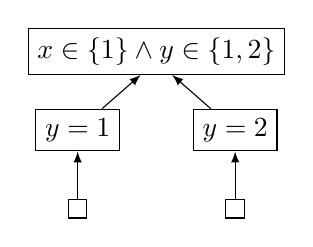
\begin{tikzpicture}
		\tikzstyle{arrow}=[draw, -latex]
		\node[rectangle,draw] at (0, 2) (levelOne) {$x \in \{1\} \land y \in \{1, 2\}$};
  		
		\node[rectangle,draw] at (-1, 1) (levelTwoElementOne) {$y = 1$};
		\coordinate[left=0.2cm of levelOne.south] (levelOnePointOne);
  		\path[arrow] (levelTwoElementOne) -- (levelOnePointOne);
		\node[rectangle,draw] at (-1, 0) (levelThreeElementOne) {\Checkmark};
  		\path[arrow] (levelThreeElementOne) -- (levelTwoElementOne);
		\node[rectangle,draw] at (1, 1) (levelTwoElementTwo) {$y = 2$};
		\coordinate[right=0.2cm of levelOne.south] (levelOnePointTwo);
  		\path[arrow] (levelTwoElementTwo) -- (levelOnePointTwo);
		\node[rectangle,draw] at (1, 0) (levelThreeElementTwo) {\Checkmark};
  		\path[arrow] (levelThreeElementTwo) -- (levelTwoElementTwo);
	\end{tikzpicture}
	\caption{search tree with constraint propagation}
	\label{fig:smallTree}
	\end{figure}
	
	To visualize this effect consider a constraint problem based on two variables $x \in \{1, 5, 6\}$ and $y \in \{1, 2\}$ and one constraint based on them.
	\begin{equation}
		c_1:\ x \le y
	\end{equation}
	Without constraint propagation and branching first on $x$ the search trees turns out to be the one in \reffig{fig:bigTree}. Obviously the right parts of this tree can already be pruned already at the root by propagation of constraint $c_1$ and therefore it is not necessary to create and evaluate these subtrees like in \reffig{fig:smallTree}.
	
	The actual implementation of constraint propagation differs again from one toolset to another, but theory underneath is the same. As the topic of this paper is the implementation in \emph{Gecode} I will concentrate on this one.
	
	Constraints in \emph{Gecode} are always evaluated ahead of a further growth of a subtree, as it may be possible to prune some of the subtrees. The problem here is to decide in which order the constraints should be considered, and it may even be necessary to evaluate some constraints more often. A short example will explain this very well \cite[p.~575]{handbookCP}: Let there be two constraints 
	\begin{equation}
		c_1: y - x^2 = 0
	\end{equation}
	\begin{equation}
		c_2: y - x - 1 = 0
	\end{equation}
	and let the variable domains be $x, y \in [-4, 4]$. Starting with the evaluation of constraint one follows a chain of reductions of the variable domains, based only on constraint propagation:
	\begin{equation}
	\begin{split}
		c_1:\ &y \in [-4, 4] \rightarrow y \in [0, 4] \\
		c_1:\ &x \in [-4, 4] \rightarrow x \in [-2, 2] \\
		c_2:\ &y \in [0, 4] \rightarrow y \in [0, 3] \\
		c_2:\ &x \in [-2, 2] \rightarrow x \in [-1, 2] \\
		c_1:\ &x \in [-1, 2] \rightarrow x \in [-1, 1.73 \dots] \\
		&\dots
	\end{split}
	\end{equation}
	
	To implement this repeated evaluation of constraints in \emph{Gecode} all constraints subscribe to the domains of the variables which are part of them. With this method the constraints get noticed whenever a variable domain is reduced and they can signal the system that they need to be evaluated once again.
	
	The next decision to be made is which constraint should be evaluated first. In the example above the constraints were quite simple and therefore it won't make a big difference to evaluate first $c_1$ or $c_2$, the search will take nearly the same time. Unfortunately not all constraints are that easy to evaluate and for this case \emph{Gecode} defines for every constraint a certain cost \cite[p.~275]{programmingGecode}. Based on this cost the constraints are sorted into buckets which are then iterated from the constraints with lower costs to the ones with higher costs. This means, whenever a variable domain is changed, the first try is to use constraints with the lowest possible cost and only if none of them needs to be evaluated constraints with higher costs are considered.
	
	\subsection{Search Algorithms}
	In constraint programming search algorithms define the way the search tree is constructed, starting from the root node. To improve the performance of the search usually at every newly created node a constraint propagation is executed to narrow the search space down. Based on these two steps then either one, the best or no solution is found. What the actual result in the end is depends on the type of search algorithm.
	
	In \emph{Gecode} it is possible to define custom strategies, but the user is supported at this point with some standard engines which can be used to build custom ones:
	\begin{itemize}
	\item Depth-First Search
	\item Limited Discrepancy Search
	\item Branch-and-Bound Search
	\item Depth-First Search Restart Optimization
	\end{itemize}
	
	In the following part I will discuss branching strategies, the Depth-first search and one of its variants, the Branch-and-bound search, the Limited-Discrepancy search as candidate for an improved backjumping-strategy, backjumping strategies in general and restart strategies.
	
	\subsubsection{Branching Strategies}
	If at one node it is not possible to empty one variable domain or to reduce all variable domains to the size one it is necessary to make a decision: How should the next subtree be constructed? The question is answered by the selected branching strategy. No matter which one is selected, they all have in common that they create additional, temporary constraints, which are only applied to the specific subtrees. This step is called \emph{posting} a constraint on a branch.
	
	The branching strategy depends on the variable domain: For Integer (and Boolean) variables there are three common strategies \cite[p.~87]{handbookCP} which differ in how the domain is distributed to the subtrees.
	\begin{itemize}
	\item Enumeration: The domain for $x \in D = {x_1, x_2, \dots}$ is split up into $|D|$-branches where for every branch $i$ one additional constraint $c:\ x = x_i$ is posted.
	\item Binary choice points: One value $x_i$ of the domain $D$ of the variable $x$ is selected and the domain is split up into two subtrees: On one the constraint $x = x_i$ and on the other one the constraint $x \ne x_i$ is posted. This results into something like a binary tree at this point.
	\item Domain splitting: The domain $D$ for the variable $x$ is split up into two disjoint intervals or sets, for example $x < 2$ and $x \ge 2$.
	\end{itemize}
	
	As for variables with a Float domain the Enumeration and Binary choice points are not feasible, the last one, domain splitting, is typically used. As termination criteria for a Float it is often necessary to define a certain epsilon $\epsilon \in \mathbb{R}_{>0}$ which describes the interval length, at which the solver states to have found a solution.
	
	For all branching strategies there is a choice of freedom left, which can be used to implement some heuristics. This additional information is either gained during the search itself of predefined by the user.
	
	\subsubsection{Depth-First Search}
	The Depth-first search is a good point to start, as it was also historical the first developed one. The idea behind this search algorithm is that every possible combination of variables is examined. Obviously in its basic form it can not be applied to problems with inifinite domains; for problems with such variable domains it is necessary to use for instance Branch-and-reduce. Sometimes the Depth-first search is also referred to as chronological backtrack search.
	
	The starting point is the root node, from where on the algorithm is called recursively. At every node mainly two steps are executed: First a constraint propagation and then a branching, which divides the search space into two disjoint sub spaces, on which the same algorithm is applied again. The search stops in a leave if either no branching is possible anymore and therefore a valid solution is found, or one or more variable domains are emptied, which indicates that in this leave no possible solution exists.
	
	This search is a so-called complete algorithm as it can be proven that all possible solutions will be found \cite[p.~85]{handbookCP}. Because of this characteristic it is very useful to proove for example that for a certain problem no solution exists. The main drawback obviously is the execution time, as it does an exhaustive search, and maybe even the memory usage if during the search many solutions are found.
	
	By stopping the search after one feasible solution is found the algorithm can often be accelerated. Although this slightly modified version is not complete anymore, in practice it is in some areas sufficient to know just one valid solution.
	
	\subsubsection{Depth-First Search with Optimization}
	If in the constraint programming an objective is defined which should be either minimized or maximized a modified version of the Depth-first search can be applied. The only difference is that it evalutes the objective function for every found solution concerning the constraints and stores during the search only the best one. To accelerate the search it is possible to add an additional constraint which defines that the new objective must better than the best so far. Through this enhancement even more sub trees are pruned and the search is faster.
	
	This algorithm is again a complete one, therefore it will always find the best solution if one exists. This algorithm does not inherit the bad memory characteristics from the Depth-first search as only one solution is stored, but the search is still exhaustive and can be very slow, depending on the size of the variable domains.
	
	\subsubsection{Branch-and-Bound Search}
	A branch-and-bound search is an algorithm for optimization of an objective function under certain constraints and only discrete possible candidates for a solution. To fulfill the constraints the first step, branch-and-reduce is applied, and the second one, bounding, is used to prune whole areas with non-optimal solutions.
	
	\begin{figure}
		\center
		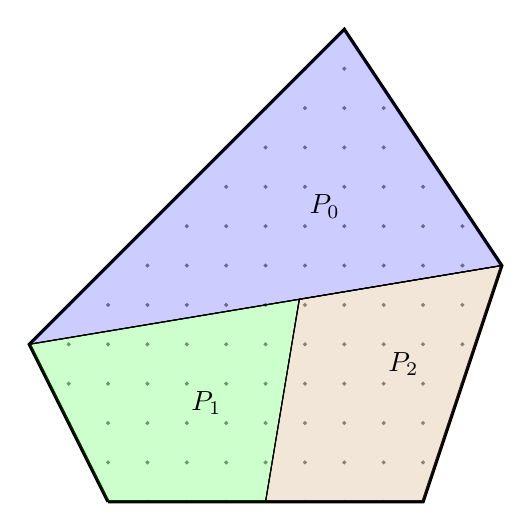
\begin{tikzpicture}
			\coordinate (a) at (0, 0);
			\coordinate (b) at (4, 0);
			\coordinate (c) at (5, 3);
			\coordinate (d) at (3, 6);
			\coordinate (e) at (-1, 2);
			\coordinate (f) at (2, 0);
			\coordinate (g) at (intersection of e--c and f--d);
			
			\begin{scope}
				\clip (a) -- (b) -- (c) -- (d) -- (e) -- (a);
				\foreach \x in {-2,-1.5,...,5}
				{
	      			\foreach \y in {0,0.5,...,6}
	      			{
	        			\node[draw,circle,inner sep=0.2pt,fill,gray] at (\x,\y) {};
	      			}
	    		}
    		\end{scope}
			
			\draw[very thick] (a) -- (b) -- (c) -- (d) -- (e) -- (a);
			\draw (a) -- (b) -- (c) -- (e) -- (a);
			\draw (f) -- (g) -- (c) -- (b) -- (f);
			\draw[fill=blue, fill opacity=0.2] (c) -- (d) -- (e) -- (c);
			\draw[fill=green, fill opacity=0.2] (a) -- (f) -- (g) -- (e) -- (a);
			\draw[fill=brown, fill opacity=0.2] (f) -- (g) -- (c) -- (b) -- (f);
			\node at (2.75, 3.75) {$P_0$};
			\node at (1.25, 1.25) {$P_1$};
			\node at (3.75, 1.75) {$P_2$};
		\end{tikzpicture}	
		\caption{Splitting of a search space into three subproblems and the possible candidates for solutions}
		\label{fig:branchAndBound}
	\end{figure}
	
	As the basic concept of the finding solutions is the enumeration of possible candidates it is necessary to seperate the search space in a useful way, which is the task for the branch-and-reduce step. Actually this step is very similar to the concept of branching, it also depends on a certain heuristic to divide the search space into two or even more disjoint parts. This heuristic can either be selected by the user or be an general one, like splitting the biggest variable domain into two equal sized parts. If the basic search space contains a big amount of possible candidate solution one reduction may not be enough and therefore this step is applied recursively to the newly create subproblems. This process can be stopped if the number of solutions is reduced to an amount, where it is possible to enumerate all of them and check if they are optimal. A possible division into subproblems can be seen in \reffig{fig:branchAndReduce}, where for legibility always only one of the subproblems is divided further.
	
	The next step after branch-and-reduce is bounding, which is able to prune whole sub problems. In the following part I will consider the minimization of an objective function without a loss of generality. For the bounding it is first necessary to initialize a upper bound with a value, for example with $\infty$. This upper bound is updated during the process every time a new optimal solution is found to this new optimum. If a new possible solution is found which is above this upper bound the algorithm can prune it, as only the minimum solution is of interest. The actually pruning of subproblems is based on the relaxed optimum, which is the optimum of the problem without consideration that only discrete values are allowed. If this relaxed optimum for a certain subproblem is greater than the current upper bound it is possible to prune this sub problem, as it can not contain a better solution.
	
	Consider for this \reffig{fig:branchAndBound}, where already a certain optimum $f$ was found in subproblem $P_1$. If now the relaxed optimum $f_{P0}$ in $P_0$ and $f_{P2}$ in $P_2$ is worse than this optimum
	\begin{equation}
		f_{P0} > f
	\end{equation}
	\begin{equation}
		f_{P2} > f
	\end{equation}
	the whole subproblems $P_{0}$ and $P_{2}$ can be pruned and it is not necessary to enumerate the solution candidates in them (or to split them further up).
	
	Combined with appropriate branching the bounding can prune several candiates at once, without the necessity to enumerate them. Therefore bounding is able to improve the performance of the search.
	
	\subsubsection{Limited Discrepancy Search}
	Limited Discrepancy Search falls into the category of Best-first searches and was first mentioned by Harvey and Ginsberg in \cite{limitedDiscrepancy}. It depends on some heurisitics for the tree, which are determined through branching strategies. The basic concept is that during a chronological backtrack search a wrong turn close to the root is first of all very expensive. Second, heuristics work worse the farther away from the solution they are applied, therefore decisions close to the root node are possible to fail. Consequently, in a chronological backtrack search the worst decisions are the most expensive ones. The Limited Discrepancy Search solves exactly this problem as it suggests to change rather the decisions made close to the root than the ones the search made later. The improvement compared to a chronological backtrack was shown by experimental results and theoretical proven in \cite{limitedDiscrepancy}.
	
	\subsubsection{Backjumping}
	A specific version of backjumping was already mentioned, the Limited Discrepancy Search, where instead of jumping one node back the algorithm always jumps as far back to the root node as possible. In general this is proven to be better than the chronological backtracking \cite{limitedDiscrepancy}, but for certain problems it may be possible to find better points to jump back. A jump back in the search tree means to detect a so-called nogood decision, which caused the violation of a constraint in the deadend. How these nogoods must be selected and stored to improve the search depends heavily on the specific field and if it is done wrong the backjumping can even be less efficient than chronological backtracking \cite[p.~100]{handbookCP}.
	
	\subsubsection{Restart Strategies}
	Branching means always to apply certain heuristics and these heuristics may fail or produce bad results for the first execution. If it turns out that the search tree is build in a disadvantageous way a restart strategy may do the trick to improve the search. For such a restart the heuristic is improved, based on the things the search has learned to be a not so good solution during the first or first few attempts to build a search tree.
	For practical application several variants of restart strategies were proposed \cite[p.~113]{handbookCP}
	
	\section{Conclusion}
	Constraint programming is a very useful tool in practice, as it can solve abritrary combinatorial or optimization problems. \emph{Gecode}, as representant of the various toolsets, implements a handy interface to transform a mathematical description of a problem into code, which then can be used to solve the problem. In conclusion, \emph{Gecode} provides all the necessary tools, combines them with a nice interface, and is still very flexible concering optimzation for a certain area through the possibility to implement custom search strategies, based on some well studied and efficient algorithms.
	
	\begin{thebibliography}{1}
		\bibitem{handbookCP}
		F.~Rossi, P.~van~Beek and T.~Walsh, \emph{Handbook of Constraint Programming}, Amsterdam, The Netherlands: Elsevier, 2006, ISBN: 978-0-444-52726-4
		\bibitem{allDifferent}
		W.~van~Hoeve, \emph{The Alldifferent Constraint: A Survey}, http://www.andrew.cmu.edu/user/vanhoeve/papers/alldiff.pdf
		\bibitem{trendsInCP}
		F.~Benhamou, N.~Jussien, B.~A.~O'Sullivan, \emph{Trends in Constraint Programming}, Wiley-ISTE, 2007, ISBN: 978-1-905209-97-2
		\bibitem{gecode}
		http://www.gecode.org/
		\bibitem{programmingGecode}
		C.~Schulte, G.~Tack and M.~Z.~Lagerkvist, \emph{Modeling and Programming with Gecode}, http://www.gecode.org/doc-latest/MPG.pdf
		\bibitem{limitedDiscrepancy}
		W.~D.~Harvey, M.~L.~Ginsberg, \emph{Limited Discrepancy Search}, Morgan Kaufmann, 1995
		\bibitem{linearProgramming}
		L.~Cooper and D.~Steinberg, \emph{Methods and Applications of Linear Programming}, W.~B.~Saunder~Company, 1974, ISBN: 0-7216-2694-7
	\end{thebibliography}
\end{document}


